\chapter{Supporting information for Chapter~\ref{chap:LLE}}
\chaptermark{SI for LLE method}
\section{Barium removal and background REE concentrations}
\sectionmark{Ba removal and REE background}

A primary objective in analyzing REE in natural water samples is the separation of Ba, which may lead to isobaric interferences with Eu.
Figure~\ref{fig:Ba-removal}A illustrates the effective rejection of Ba by the LLE method presented here, however Figure~\ref{fig:Ba-removal}C shows that even with $\sim0.2\%$ \ce{^{135}Ba^{16}O+}:\ce{^{135}Ba+}, the \ce{^{151}Eu+} is indistinguishable from \ce{^{135}Ba^{16}O+} in the vast majority of samples prior to barite precipitation.
Following precipitation (Figures~\ref{fig:Ba-removal}B,D), these issues are resolved.

\begin{figure}[htbp]
\begin{center}
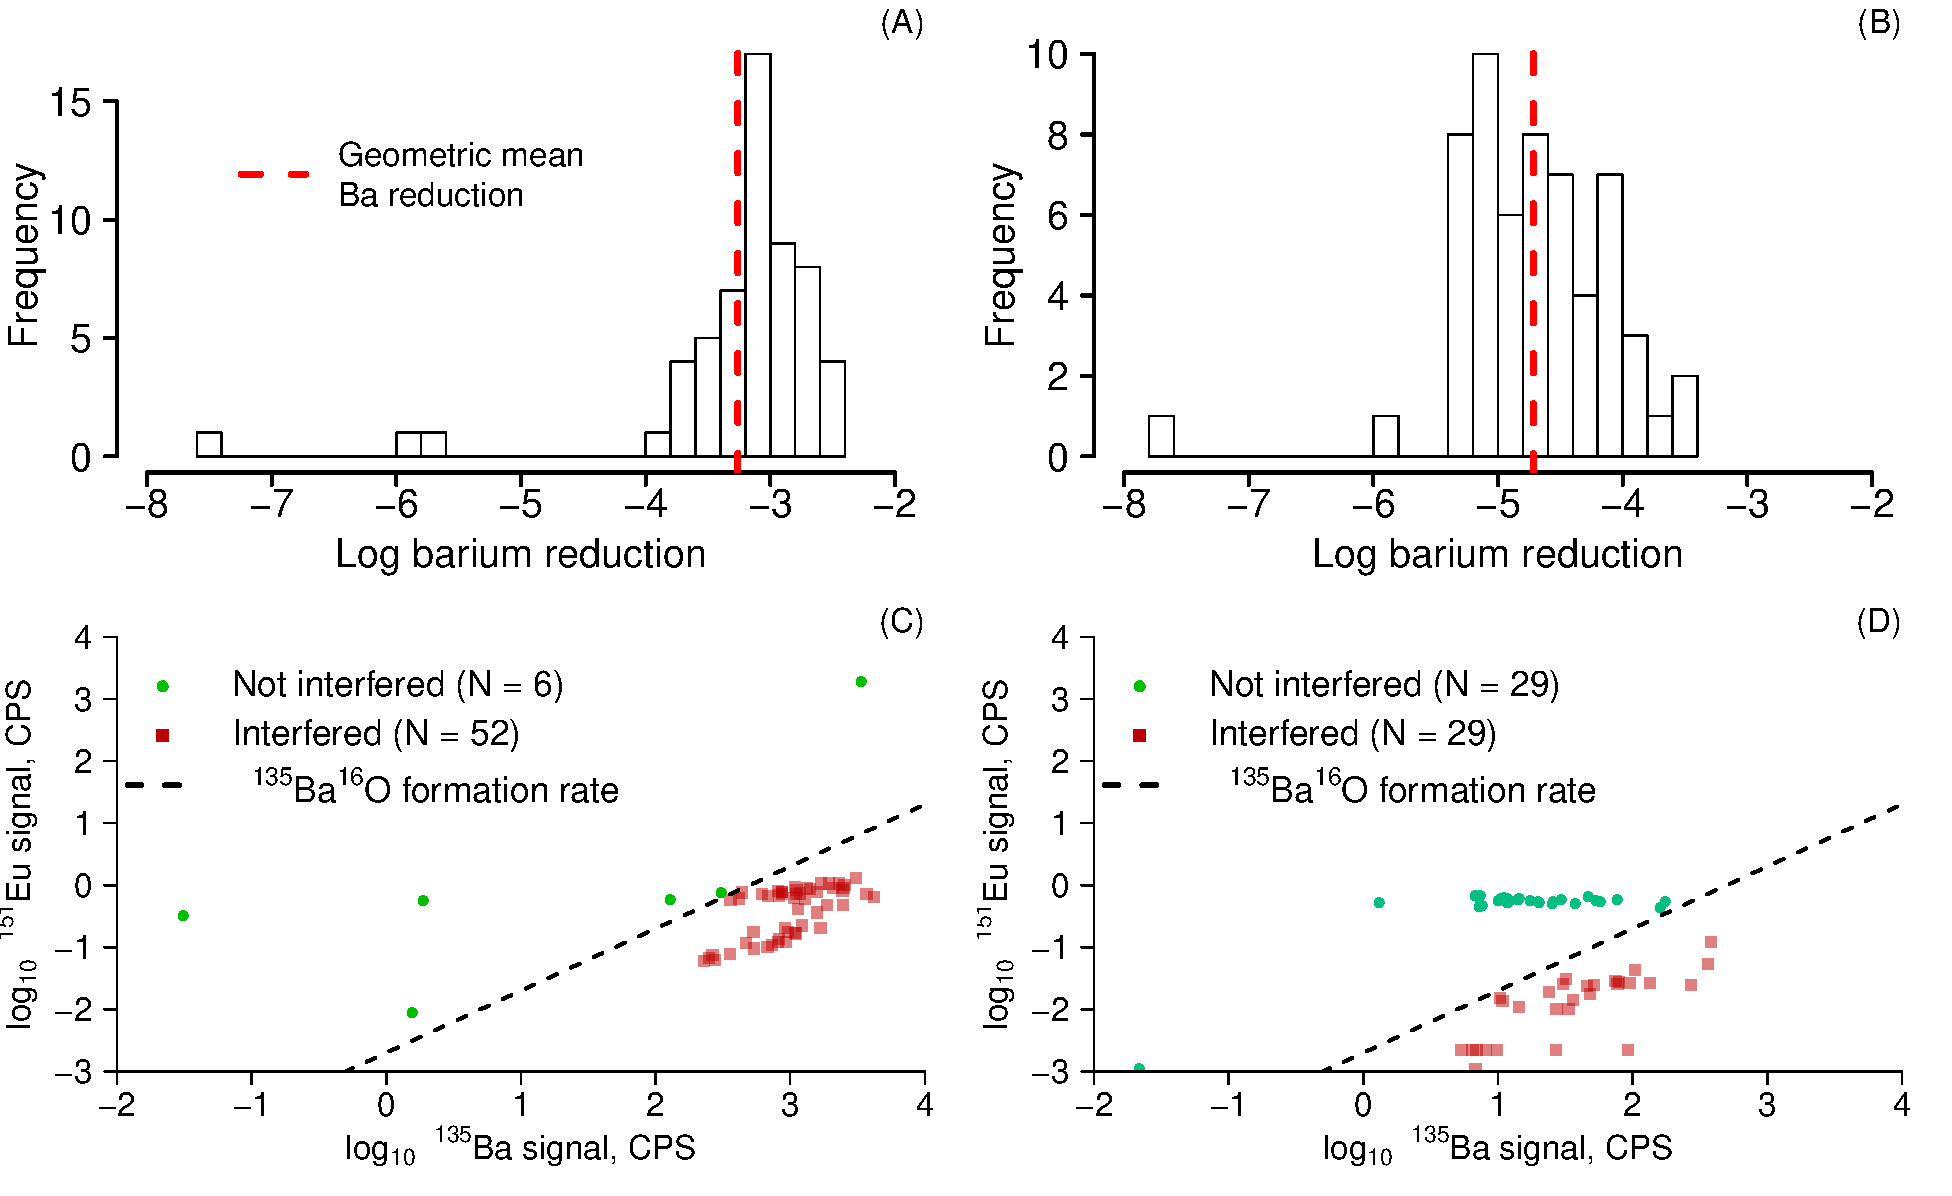
\includegraphics[width=0.8\textwidth]{Ch4_figures/Ba-removal.pdf}
\caption{Efficiency of Ba removal by LLE method (A, C) and ICP-MS octopole collision cell (B, D).
Results are for samples without (A, C) and with (B, D) \ce{H2SO4} addition to precipitate barite.
In (B) and (D), \ce{^{135}Ba^{16}O+} rate is inferred from 23 replicate analyses of a 200 ppb Ba standard after blank subtraction.
Interfered samples are those where accurate Eu determination could not be made due to excessive \ce{^{135}Ba^{16}O+} interference. In (D) the interfered samples were all unspiked experiments.}\label{fig:Ba-removal}
\label{default}
\end{center}
\end{figure}

Other experimental work in our shared lab space involves high concentrations ($\sim$mM) of Gd.
We ascribe the uniformly high Gd background in all experiments to cross contamination in this shared space.
In the ``Blank'' experiment (i.e. pH adjusted ASTM Type I water), all analytes were below detection (IDL $\sim$ 5 -- 20 ppt for 1\% false negative rate) except for Ba, La, and Gd. 
This indicates that the high La background could either be a result of laboratory cross-contamination (as with Gd) or an impurity in the organic phases used.
The latter supposition was investigated by direct contact of the mixed organic phases used (i.e. 3 mL 0.25 M HDEHP in heptane  + 1 mL octanol) with 4 mL of 6 N HCl, followed by analysis of the acid phase.
These results were below detection (not pictured), indicating no significant REE contamination of the organic phases.
While all chemicals were purchased at high purity, we can assume that the observed background concentrations in other experiments are due to trace contamination of these reagents.
Paradoxically, the level of these contaminations cannot be determined by ICP-MS without applying a separation/preconcentration technique such as the LLE method;
this makes source apportionment of the observed background concentration challenging.

\begin{sidewaysfigure}[htbp]
\begin{center}
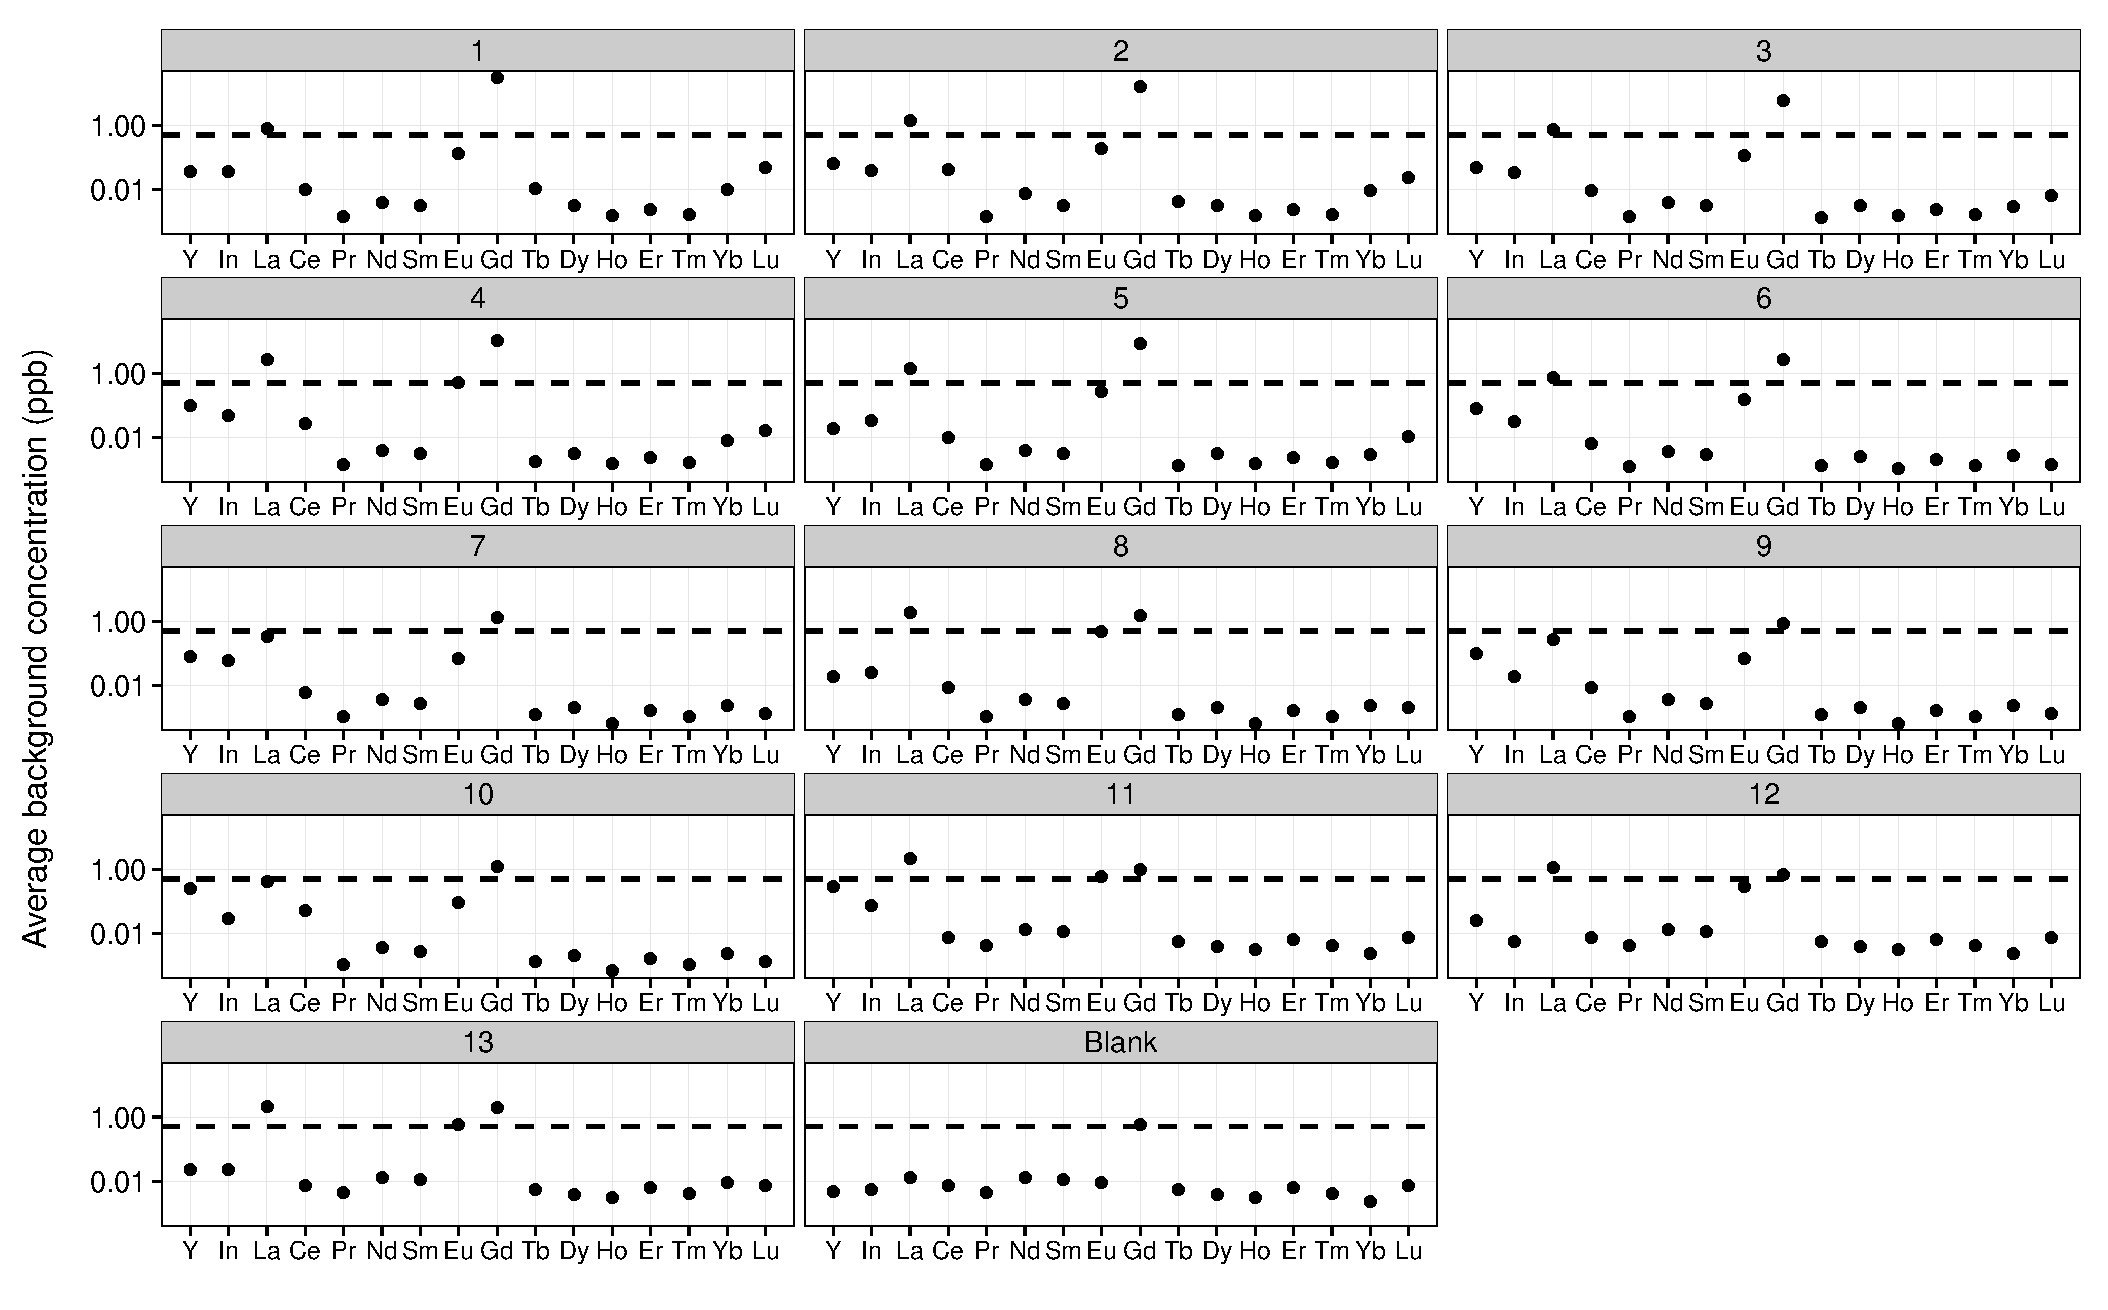
\includegraphics[width=0.95\textwidth]{Ch4_figures/REE-bkgd.pdf}
\caption{Average (from $n \geq 2$ replicates, except for Blank and experiments 6, 13) background concentrations of target analytes in samples without \ce{BaSO4} precipitation.
Dashed line at 500 ppt indicates the input concentration for all spiked samples.
Note that the y-axis is a logarithmic scale. Blank experiment represents pH adjusted ASTM Type I water.}\label{fig:REE-bkgd}
\end{center}
\end{sidewaysfigure}

\clearpage

\section{Doehlert experimental results}

These data represent the experiment and replicate ordered results of Doehlert matrix tests.
Each experiment number represents a unique set of solution conditions ([NaCl], [Fe], and [DOC]);
values for each of these parameters in each experiment is given in Table~\ref{tab:Doehlert}.

\begin{sidewaysfigure}[htbp]
\begin{center}
\includegraphics[width=\textwidth]{Ch4_figures/Exp-wise-LLE-recovery.pdf}
\caption{Elemental recovery in Doehlert matrix samples by LLE methodology (see Table~\ref{tab:Doehlert} for experimental conditions).
Recovery values for Eu were determined after dosing the LLE eluent with \ce{H2SO4} to precipitate barite;
all other recoveries were determined without barite precipitation.
Elements where the background concentration was determined to 250 ppt or greater (see Figure~\ref{fig:REE-bkgd}) were excluded (i.e. La and Gd in all experiments and Y in experiment 11).}
\label{fig:Doehlert-all}
\end{center}
\end{sidewaysfigure}

